\chapter{Rover Model Development Methodology}
\section{Development Objectives}
  \subsection{Problem Definition}
  The project aimed to propagate the theme of science education and outreach, leveraging the modern technologies of today, through the development of a working, scaled down version of the \textit{Curiosity} rover. The project brief indicated that the typical use case as desired by the client was to have the rover simulate chosen, significant features of the rover on Mars to shed some light on the level of capability of space technologies that are currently in operation. The model will be set either in a simulated Martian environment or in a small display area and be required to be remotely controllable, providing video and telemetry to viewers and viewer's devices the same way the RSVP would to the flight team at JPL.
  
  As an initiation of the project, the requirements were explored and collated below into a list of those pertaining to the vehicle itself in a sense of the hardware as well as the software that encompassed the operation of the vehicle as an educational piece. The requirements made sure to maintain as little reference to technologies available as possible as this detail was to be further developed after analysis of the requirements on a functional level.
  
  \subsection{Project Requirements}
  \begin{enumerate}
    \item Develop and build a model of the Mars \textit{Curiosity} rover. The rover model should:
    \begin{enumerate}
      \item\label{enum:req-scaledrover} be a scaled down representation of JPL's rover currently operational on Mars with a level of resemblance adequate for use in a realistic exhibit. In other words, it should have been realistic enough such that someone who might have seen a picture of \textit{Curiosity} beforehand could identify the rover,
      \item have traversal capabilities that reflect those on \textit{Curiosity},
      \item be able to make use of these traversal capabilities on uneven terrain such as one which would be a simulated surface as part of the exhibit without resulting in an unrecoverable state,
      \item have reasonable awareness of obstacles to prevent resulting in an unrecoverable state as well as to provide an indication of the navigational and environmental awareness systems on \textit{Curiosity},
      \item have data communication facilities available to best represent the communication systems and subjects of those that are a part of MSL, and
      \item be completely wireless, again reflecting the nature of operation of \textit{Curiosity}.
    \end{enumerate}
    \item Develop a software system to accompany the above rover in its functioning. The software system should:
    \begin{enumerate}
      \item be able to receive data in the form of video and telemetry from the model,
      \item be able to present the data received to users or operators in an interactive manner on a platform that is available and accessible,
      \item allow input of commands or control by the users in a manner which is both friendly to a wide range of audiences and age groups and as closely representative of the manner in which JPL's flight team would do so,
      \item transmit these commands to the model to be executed, and
      \item facilitate the reception and transmission of the above data wirelessly.
    \end{enumerate}
  \end{enumerate}
  
  \subsection{Analysis of Constraints}
    As with any engineering design project, the rover development was faced with multiple constraints that affected the resulting design. Below is a brief list of the constraints known at the beginning of the project.
    
    \begin{itemize}
      \item Typical exhibition space limited to a dimension of 3m x 3m
      \item 
    \end{itemize}
    
  \subsection{Functional Analysis}
    The client requirements as highlighted in the previous sub-section were analysed to result in a functional outline in lieu of developing a list of specifications. This analysis served as the starting point for the componentization of the project, allowing for the conceptual development to follow the breakdown. This is discussed further in the next section. Here, each of the requirements, and combinations of them, were used to result in a breakdown of functions and aspects. A significant effort was made from the start of the project to develop the rover in a modular fashion. This is not to be confused with the outcome being modular (although this was still a desirable feature) but rather the way in which ideas were formed and developed. The functions outlined in this analysis were treated as modules, where possible, and developed so that each module had as little dependence in operation as possible on another. Following this mindset allowed for the simplification of the design process and the robustness of what was developed against constraints and unforeseen obstacles during development.
    
    The current requirements distinguished clearly the two aspects of the project which inevitably became the two major points of development. Both aspects, the mechanical vehicle and the software system, and their differing associated design approaches made it suitable to discuss them separately, where appropriate.
    
    \begin{figure}[h]
      \centering
      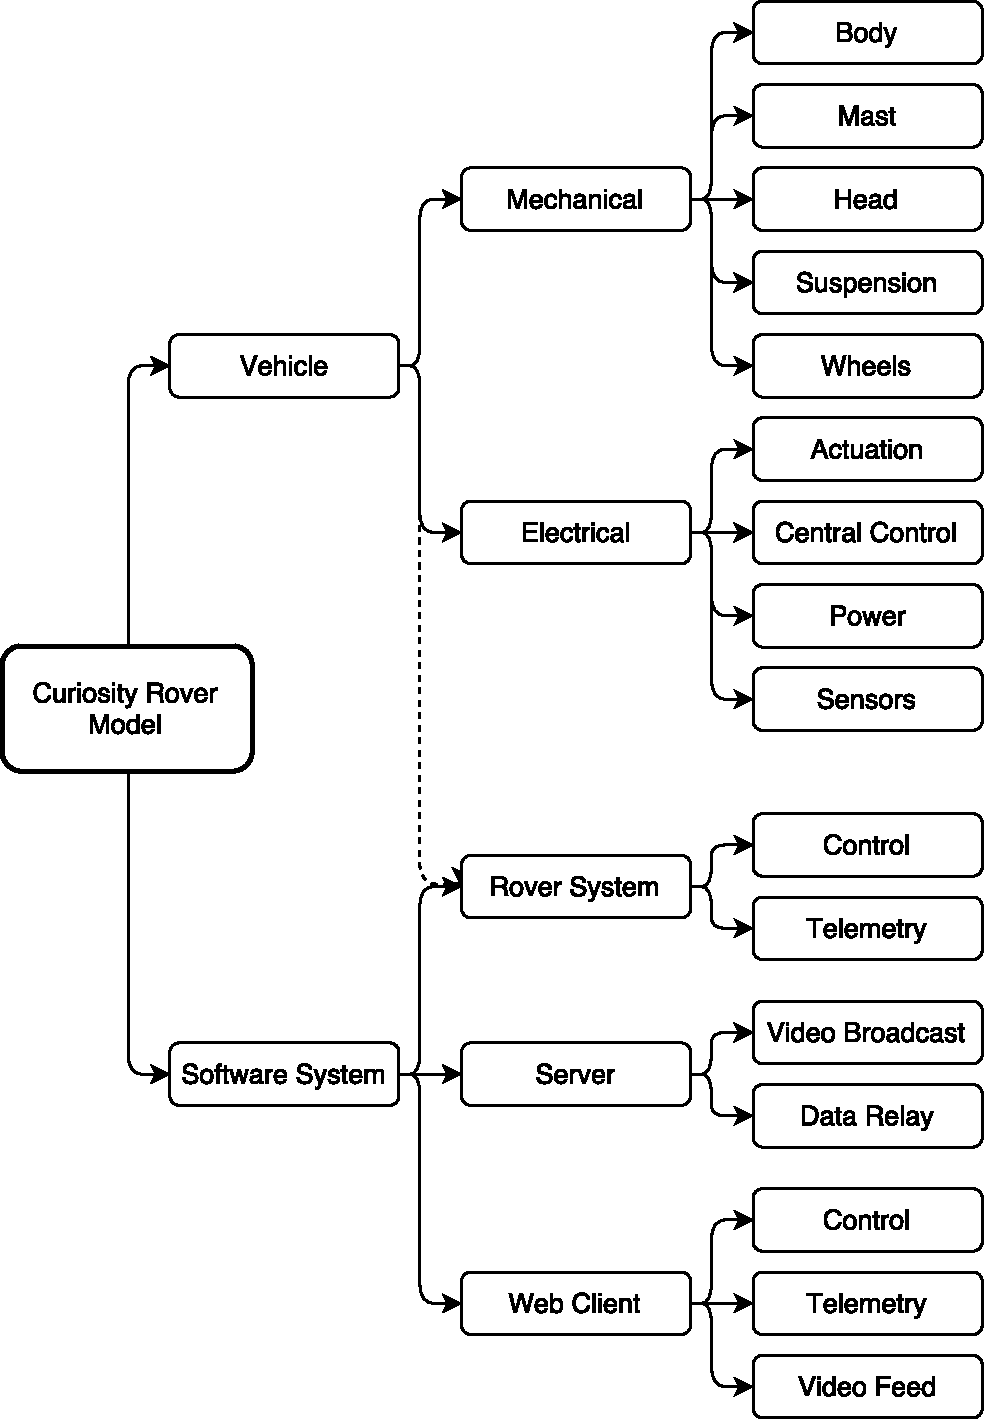
\includegraphics[width=0.6\textwidth]{figures/specs-functionalBreakdown}
      \label{fig:specs-functionalBreakdown}
      \caption[Diagram showing the simplified breakdown of functional entities of the project]{Diagram showing the simplified breakdown of functional entities of the project}
    \end{figure}
    
    
  \subsection{Technical Specifications}
    The technical specifications were derived from the client requirements and the functional analysis, with knowledge of the systems and subsystems on \textit{Curiosity} (taken from review of literature as covered in Chapter~\ref{chap:lit-review}). The specifications further compartmentalised the vehicle and software systems as evident in the structure of them in the lists that follow. These technical specifications served as the baseline requirements for the final design. Section~\ref{sec:secondary-objectives} adds to the these specifications a list of secondary objectives which were considered during the design process, but not mandatory.
    
    
  
  \subsection{Secondary Objectives}
  \label{sec:secondary-objectives}